\chapter{Square-Wave Phase Grating}
\label{app:SWPG}

\begin{equation}
\begin{aligned}
I_{IR} &= a + b\times\cos\left(\phi(x_{0})\right)\\
I_{q} &= \alpha_q\times a^{q} \left(1+N_{q}\frac{b}{a}\cos\left(\phi(x_{0})\right)\right) + o(b\times a^{q-1})\\
\end{aligned}
\end{equation}
\begin{equation}
\begin{aligned}
I_{IR}(\tilde{x}_{1},x_{0}) &= \left|\tilde{S}(\tilde{x}_{1},x_{0})\right|^{2} \\
&= \left|a_{-1}\tilde{E}(2\tilde{x}_{1})+a_{0}\tilde{E}(\tilde{x}_{1})+a_{1}\tilde{E}(0)+a_{3}\tilde{E}(2\tilde{x}_{1})\right|^{2}\\
&= \left|a_{0}\tilde{E}(\tilde{x}_{1})+a_{1}\tilde{E}(0)\right|^{2}\\
\end{aligned}
\end{equation}
\begin{equation}
\begin{aligned}
I_{IR}(\tilde{x}_{1},x_{0}) &=\left|\tilde{E}(0)\right|^{2}\left|\frac{2}{\pi}\sin\left(\xi\frac{\pi}{2}\right)e^{i(\xi\frac{\pi}{2}-\phi_{1})}+\cos\left(\xi\frac{\pi}{2}\right)e^{i\xi\frac{\pi}{2}}\frac{\tilde{E}(\tilde{x}_{1})}{\tilde{E}(0)} -  \frac{2\sin\left(\xi\frac{\pi}{2}\right)}{\pi}e^{i(\xi\frac{\pi}{2}+\phi_{1})}\frac{\tilde{E}(2\tilde{x}_{1})}{\tilde{E}(0)} + \frac{2\sin\left(\xi\frac{\pi}{2}\right)}{3\pi}e^{i(\xi\frac{\pi}{2}-3\phi_{1})}\frac{\tilde{E}(2\tilde{x}_{1})}{\tilde{E}(0)}\right|^{2}\\
\end{aligned}
\end{equation}
\begin{equation}
\begin{aligned}
I_{IR}(\tilde{x}_{1},x_{0})  &= \left|\tilde{E}(0)\frac{2}{\pi}\sin\left(\xi\frac{\pi}{2}\right)\right|^{2}\left|e^{-i\phi_{1}}+\frac{\pi}{2\tan\left(\xi\frac{\pi}{2}\right)}\frac{\tilde{E}(\tilde{x}_{1})}{\tilde{E}(0)} -e^{i\phi_{1}}\frac{\tilde{E}(2\tilde{x}_{1})}{\tilde{E}(0)} +  \frac{e^{-3i\phi_{1}}}{3}\frac{\tilde{E}(2\tilde{x}_{1})}{\tilde{E}(0)}\right|^{2}\\
&= \left|\tilde{E}(0)\frac{2}{\pi}\sin\left(\xi\frac{\pi}{2}\right)\right|^{2}\left(1+\frac{\pi}{\tan\left(\xi\frac{\pi}{2}\right)}\frac{\tilde{E}(\tilde{x}_{1})}{\tilde{E}(0)}\cos(\phi_{1})-\frac{4}{3}\frac{\tilde{E}(2\tilde{x}_{1})}{\tilde{E}(0)}\cos(2\phi_{1})\right)\\
I_{IR}(\tilde{x}_{-1},x_{0}) &= \left|\tilde{S}(\tilde{x}_{-1},x_{0})\right|^{2} \\
&= \left|a_{-1}\tilde{E}(0)+a_{0}\tilde{E}(\tilde{x}_{1})\right|^{2}\\
&= \left|\tilde{E}(0)\right|^{2}\left|-\frac{2}{\pi}\sin\left(\xi\frac{\pi}{2}\right)e^{i(\xi\frac{\pi}{2}+\phi_{1})}+\cos\left(\xi\frac{\pi}{2}\right)e^{i\xi\frac{\pi}{2}}\frac{\tilde{E}(\tilde{x}_{1})}{\tilde{E}(0)}+\frac{2\sin\left(\xi\frac{\pi}{2}\right)}{\pi}e^{(\xi\frac{\pi}{2}-\phi_{1})}\frac{\tilde{E}(2\tilde{x}_{1})}{\tilde{E}(0)} -  \frac{2\sin\left(\xi\frac{\pi}{2}\right)}{3\pi}e^{(\xi\frac{\pi}{2}+3\phi_{1})}\frac{\tilde{E}(2\tilde{x}_{1})}{\tilde{E}(0)}\right|^{2}\\
&= \left|\tilde{E}(0)\frac{2}{\pi}\sin\left(\xi\frac{\pi}{2}\right)\right|^{2}\left|e^{-i\phi_{1}}-\frac{\pi}{2\tan\left(\xi\frac{\pi}{2}\right)}\frac{\tilde{E}(\tilde{x}_{1})}{\tilde{E}(0)} -e^{i\phi_{1}}\frac{\tilde{E}(2\tilde{x}_{1})}{\tilde{E}(0)} +  \frac{e^{-3i\phi_{1}}}{3}\frac{\tilde{E}(2\tilde{x}_{1})}{\tilde{E}(0)}\right|^{2}\\
&= \left|\tilde{E}(0)\frac{2}{\pi}\sin\left(\xi\frac{\pi}{2}\right)\right|^{2}\left(1-\frac{\pi}{\tan\left(\xi\frac{\pi}{2}\right)}\frac{\tilde{E}(\tilde{x}_{1})}{\tilde{E}(0)}\cos(\phi_{1})-\frac{4}{3}\frac{\tilde{E}(2\tilde{x}_{1})}{\tilde{E}(0)}\cos(2\phi_{1})\right)\\
%\forall n \in \mathbb{Z}, a^{\xi}_{2n+1}(x_{0}) &= \frac{2\sin\left(\xi\frac{\pi}{2}\right)}{(2n+1)\pi}e^{i(\xi\frac{\pi}{2}-(2n+1)\phi_{1})} \\
a^{\xi}_{0}(x_{0}) &= \cos\left(\xi\frac{\pi}{2}\right)e^{i\xi\frac{\pi}{2}}
\end{aligned}
\end{equation}

\begin{figure}
	\centering
	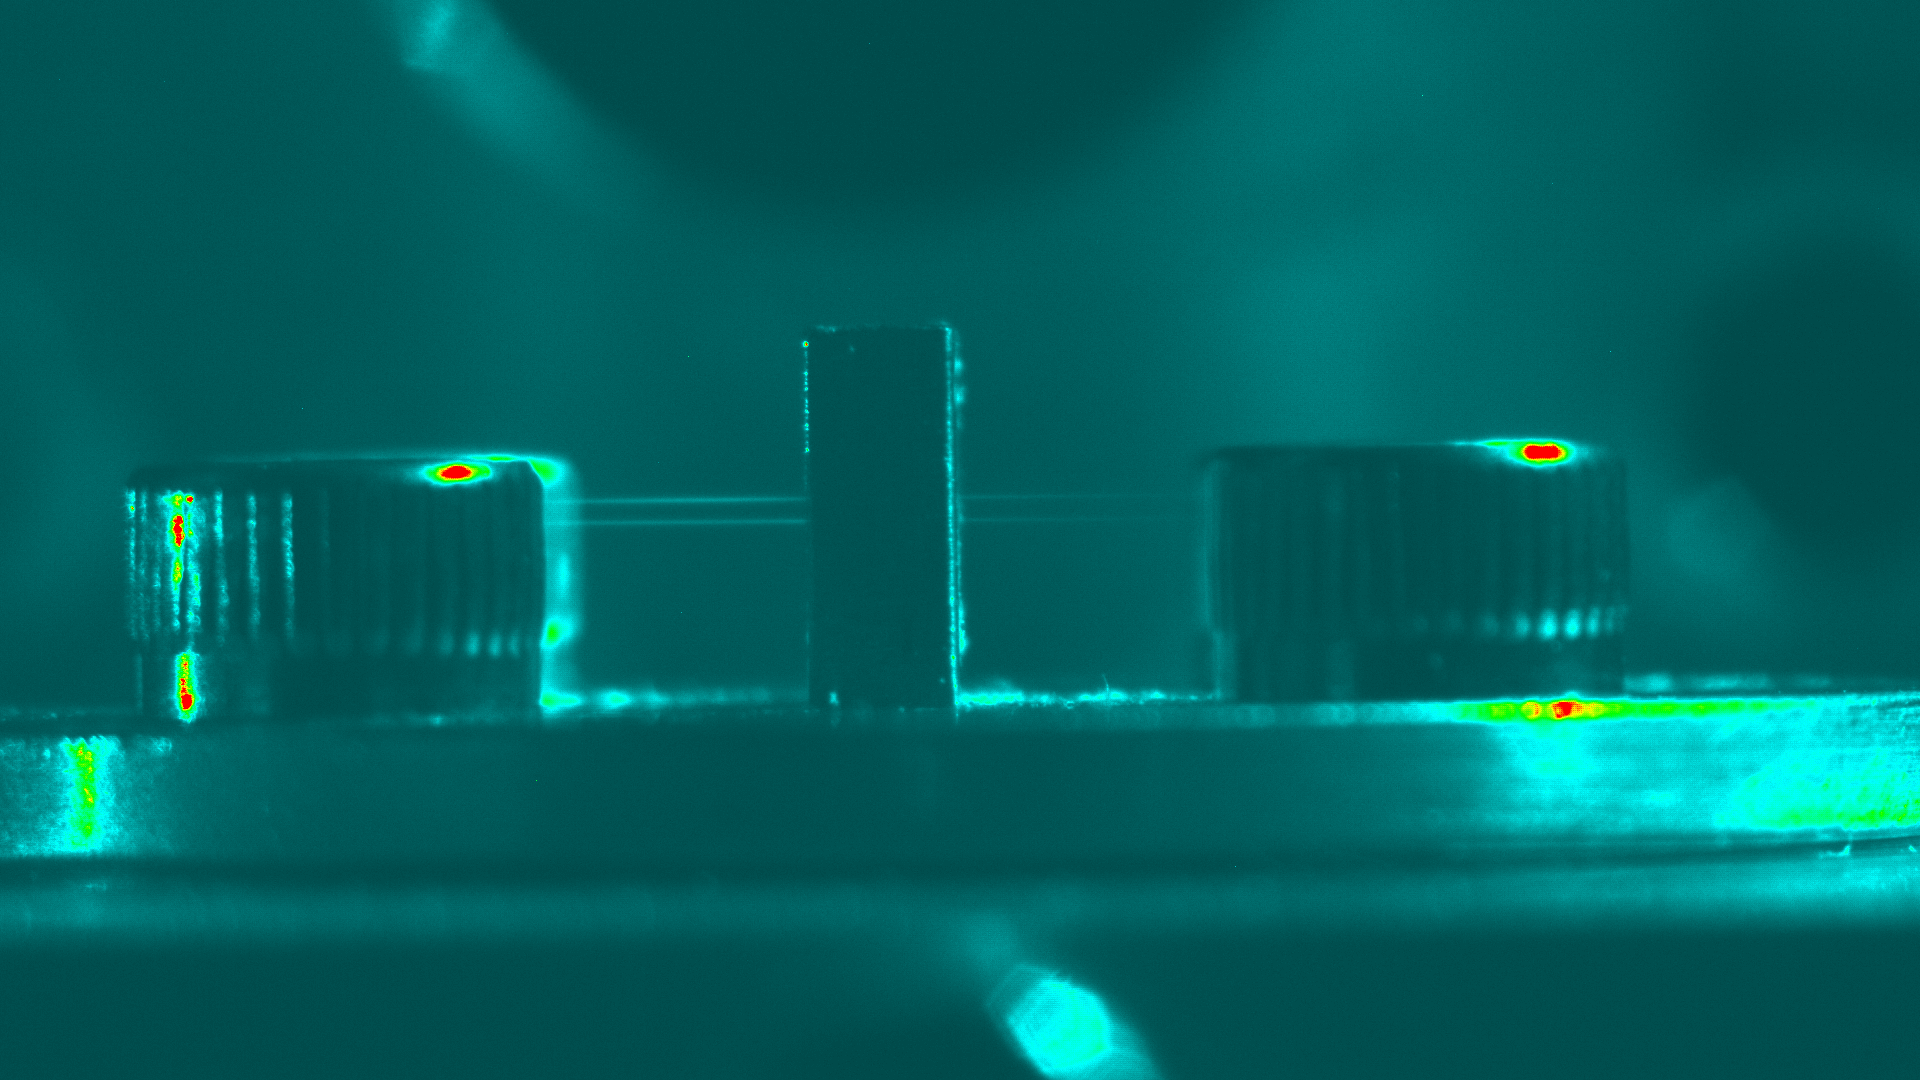
\includegraphics[width=0.9\textwidth]{figures/Two_source/ts_filament_gas_cell.png}
	\caption{Camera image of two sources generating a filament in a gas cell. Image was taken while chamber was vented and at ambient pressure.}
	\label{ts_filament}
\end{figure}


\begin{figure}
	\centering
	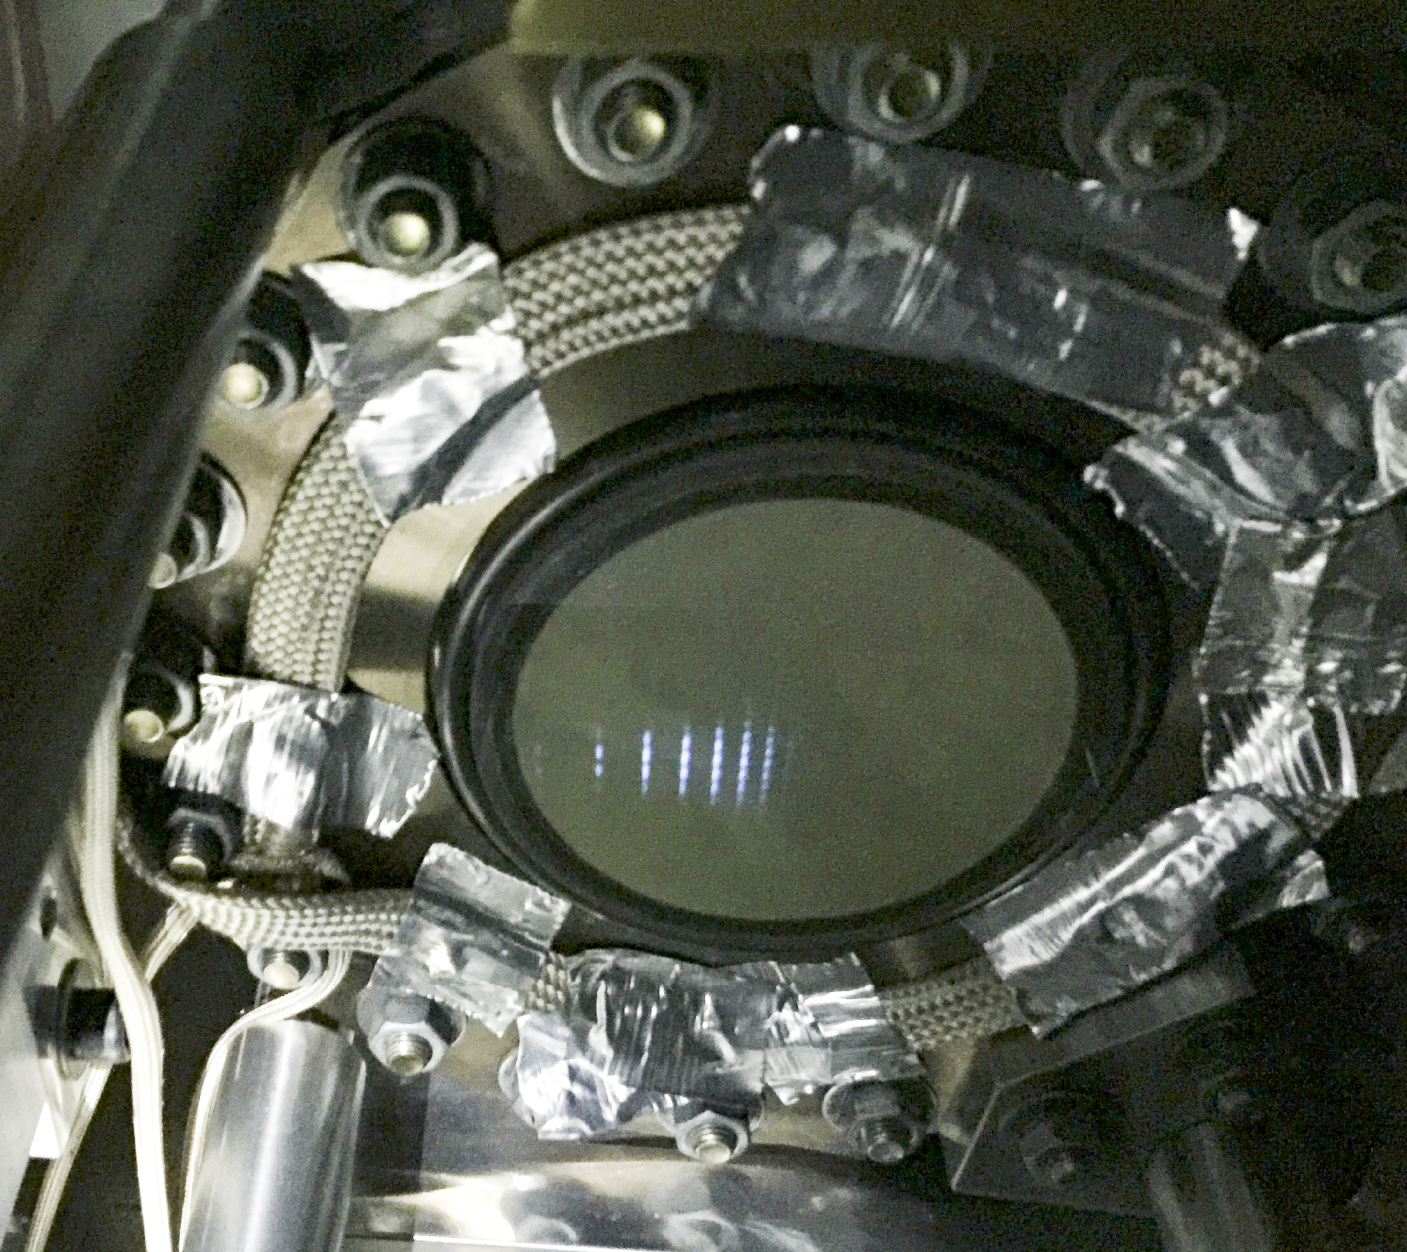
\includegraphics[width=0.6\textwidth]{figures/Two_source/MCP_ts_harmonics.png}
	\caption{Camera image of the output of the phosphor screen.  Harmonics are visible by eye.}
	\label{MCP_ts_harmonics}
\end{figure}

